% Afficher des recommendations concernant la syntaxe.
\RequirePackage[orthodox,l2tabu]{nag}
\RequirePackage{luatex85}
% Paramètres du document.
\documentclass[%
a5paper%                       Taille de page.
,11pt%                         Taille de police.
,DIV=15%                       Plus grand => des marges plus petites.
,titlepage=on%                 Faut-il une page de titre ?
%,headings=optiontoheadandtoc%  Effet des paramètres optionnels de section.
%,headings=small%
,parskip=false%
,openany%
]{scrbook}
\renewcommand*\partheademptypage{\thispagestyle{empty}}
\newcounter{facteur}\setcounter{facteur}{17}%%%%%%%%%%%%%% Paramètre pour la taille globale des partitions. par défaut~: 17
%\usepackage{geometry}
\usepackage{gredoc,mudoc,lyluatex}
\usepackage{pdfpages,transparent,array,ltablex}
\usepackage{framed}

%%%%%%%%%%%%%%%%%%%%%%% Paramètres variables %%%%%%%%%%%%%%%%%%%%%%%%%%%%%%%%%%%%%%%%%%%%%%%%%%
%%% Taille des partitions grégoriennes.                                                      %%
\grechangedim{overhepisemalowshift}{.7mm}{scalable}
\grechangedim{hepisemamiddleshift}{1.4mm}{scalable}
\grechangedim{overhepisemahighshift}{2.1mm}{scalable}
\grechangedim{vepisemahighshift}{2.1mm}{scalable}
%\grechangestafflinethickness{50} %%% epaisseur des lignes
\grechangestaffsize{\value{facteur}}%%%%% 
%%%%%%%%%%%%%%%%%%%%%%%%%%%%%%%%%%%%%%%%%%%%%%%%%%%%%%%%%%%%%%%%%%%%%%%%%%%%%%%%%%%%%%%%%%%%%%%
% Par souci de clarté, la définition des commandes est reportée dans un document annexe.

\addtolength{\voffset}{2mm}\addtolength{\headsep}{-2mm}
\setlength{\extrarowheight}{2mm}
\addto\captionsfrench{%
  \renewcommand{\indexname}{Index des chants}%
}

\pdfcompresslevel=9

\newcommand{\lieu}[1]{\hfill\linebreak[3]\hspace*{\stretch{1}}\nolinebreak\mbox{\emph{(#1)}}}

\newcommand{\commandement}[1]{\noindent\textbf{#1}}

\newcommand{\schola}[1]{}\newcommand{\foule}[1]{#1}
\providecommand{\dest}{foule}%

\newcommand{\bgimage}[1]{%image d'arrière plan
    \raisebox{-.45\paperheight}[0pt][0pt]{%
      \transparent{0.3}%
      \includegraphics[width=.7\paperwidth,height=.7\paperheight,keepaspectratio=true]{img/#1}%
      }%
}

\def\arraystretch{1.2}

\newcommand{\reponsegras}[2]{
    \versio{\textbf{#1}}{{#2}}
}
\newcommand{\imagecentre}[2]{
\begin{center} \includegraphics[height=#1]{img/#2} \end{center}}

\title{Jubilé de Notre-Dame de Fontpeyrine}
\date{}

\let\oldaddchap\addchap
\def\addchap#1{\oldaddchap{#1}\markright{Mariage}}

\def\blindsection#1{\markright{#1}\addcontentsline{toc}{section}{#1}}
%%%%%%%%%%%%%%%%%%%%%%%%%%%%%%%%%%%%%%%%%%%%%%%%%%%%%%%%%%%%%%%%%%%%%%%%%%%%%%%%
%%%%%%%%%%%%%%%%%%%%%%%%%%%%%%%%%%%%%%%%%%%%%%%%%%%%%%%%%%%%%%%%%%%%%%%%%%%%%%%%
%%%%%%%%%%%%%%%%%%%%%%%%%%%%%%%%%%%%%%%%%%%%%%%%%%%%%%%%%%%%%%%%%%%%%%%%%%%%%%%%
\begin{document}

%\maketitle
%{\pagestyle{empty}
%\foule{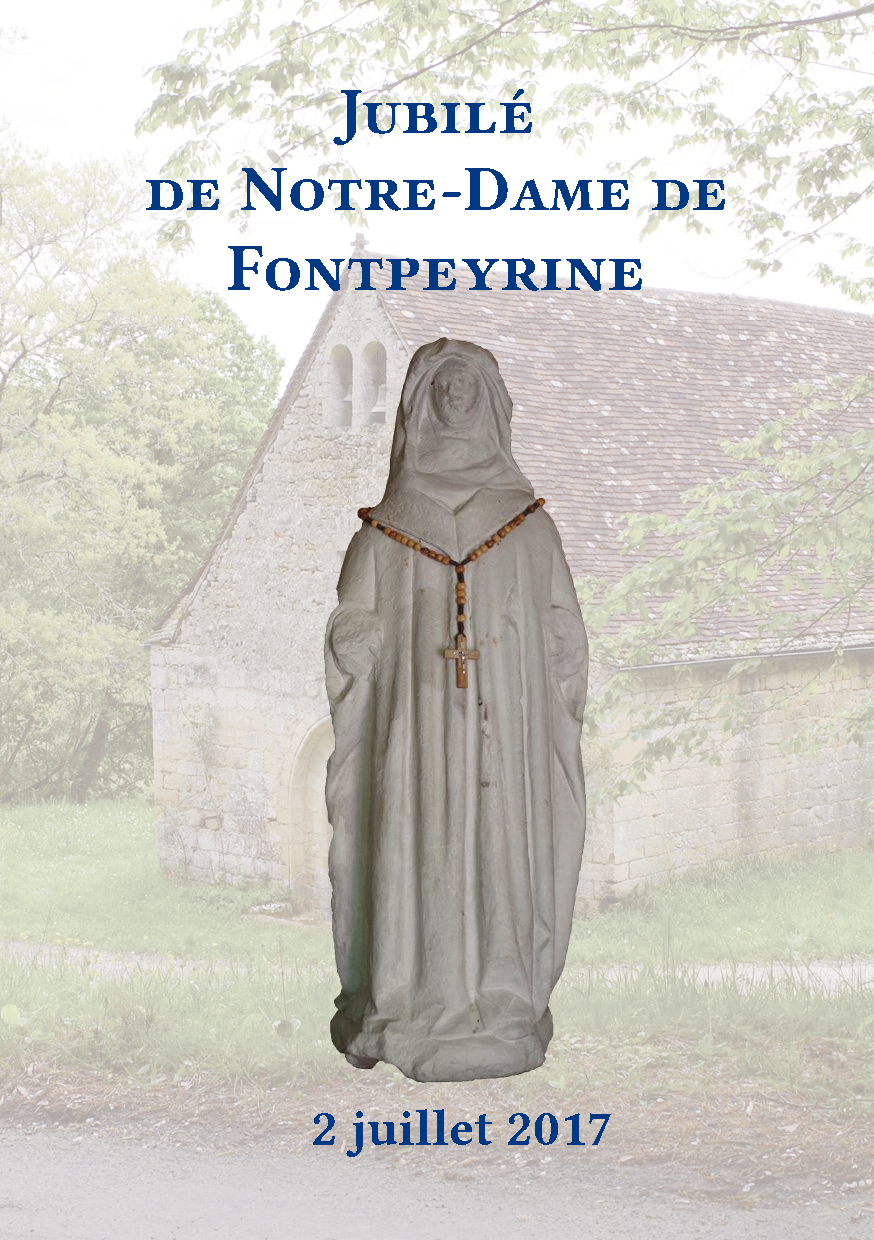
\includepdf{img/Couverture}}
%\schola{\includepdf{Couverture-schola}}
%\clearpage}
%%%%%%%%%%%%%%%%%%%%%%%%%%%%%%%%%%%%%%%%%%%%%%%%%%%%%%
\thispagestyle{empty}
\vspace*{\stretch{1}}
\begin{center}
\begin{itshape}
{
Chers amis,

\vspace*{3cm}
Cette messe à laquelle vous allez vous unir par la prière sera célébrée selon le rite traditionnel catholique de Saint Pie V.

\medskip
Par respect pour le Saint Sacrifice de la Messe et dans l'observance de la tradition de l'Église Catholique, les prières seront dites en latin.

\medskip
La célébration du mariage comprend divers éléments.

\medskip
L'essentiel est le \emph{sacrement} lui-même, que les fiancés se donnent l'un à l'autre au pied de l'autel devant l'Église, en la personne de l'un de ses prêtres dûment autorisé.

\medskip
Cette union sacramentelle se réalise par la mutuelle donation que les fiancés se font eux-mêmes, donation qu'ils expriment par un acte d'acceptation réciproque : le \emph{«oui»} qui les engage.
La cérémonie de l'union des mains, suivie de la remise de l'anneau, est le signe du secours mutuel que les époux se doivent et du lien qui par la grâce de Dieu, les unit.}
\end{itshape}
\end{center}

\vspace*{\stretch{1}}

\newpage
\subsection*{Veni Creator}
\rubrica{La cérémonie commence par l'invocation du Saint-Esprit.}
\rubrica{On se met à genoux pour la première strophe. L'hymne est alterné avec la chorale.}
\cantus{Hymne}{VeniCreator-intonation}{Hymn.}{8}
\vulgo{1. Venez Esprit Créateur, visitez les âmes de vos fidèles, comblez de la grâce d'en haut les Cœurs que vous avez créés.}
\noindent
\versio{%
2. Qui díceris Paráclitus,\\
Altíssimi donum Dei,\\
Fons vivus, ignis, cáritas\\
Et spiritális únctio.}{%
\small {2. Vous qu'on appelle Conso\-lateur, don du Dieu très-haut, source vive, feu, charité et onction spirituelle.}}

\versio{%
3. Tu septifórmis múnere,\\
Dig\textit{i}tus patérnæ déxteræ,\\
Tu rite promíssum Patris,\\
Sérmone ditans gúttura.}{%
\small {3. Vous l'Esprit aux sept dons, le doigt de Dieu, la promesse authentique du Père, qui mettez sa parole sur nos lèvres.}}

\versio{%
4. Accénde lumen sénsibus,\\
Infúnd\textit{e} amórem córdibus,\\
Infírma nostri córporis\\
Vírtute firmans pérpeti.}{%
\small {4. Eclairez nos esprits de votre lumière, mettez l'amour dans nos cœurs~; soutenez la faiblesse de notre corps par votre constante vigueur.}}

\versio{%
5. Hostem repéllas lóngius,\\
Pacémque dones prótinus~:\\
Ductóre sic te pr\'\ae vio\\
Vitémus omne nóxium.}{%
\small {5. Chassez l'ennemi loin de nous, donnez-nous sans retard la paix~; guidez-nous, et que sous votre conduite nous évitions tout mal.}}

\versio{%
6. Per te sciámus da Patrem,\\
Noscámus atque Fílium,\\
Tequ\textit{e} utriúsque Spíritum\\
Credámus omni témpore.}{%
\small {6. Faites-nous connaître le Père, faites-nous connaître le Fils, donnez-nous de toujours croire en vous qui êtes l'Esprit du Père et du Fils.}}

\versio{%
7. Deo Patri sit glória,\\
Et Fílio qu\textit{i} a mórtuis\\
Surréxit, ac Paráclito,\\
In sæculórum s\'\ae cula. Amen.}{%
\small {7. Gloire soit à Dieu le Père, et au Fils ressuscité des morts, et à l'Esprit consolateur dans les siècles des siècles. Ainsi soit-il.}}

\versio{%
\vb\ Emítte Spíritum tuum, et creabúntur}{%
\vb\ Envoyez votre Esprit, Seigneur, et il se fera une création nouvelle.}
\reponsegras{%
\rb\ Et renovábis fáciem terræ}{%
\rb\ Et vous renouvellerez la face de la terre.}

\versio{Orémus.\par\nopagebreak}{Prions.\par\nopagebreak}
\versio{Deus, qui corda fidélium Sancti Spíritus illustratióne docuísti : da nobis in eódem Spíritu recta sápere, et de eius consolatióne gaudére. \Perdominum{ }\quitecum{ }\peromnia. \mbox{\textbf{℟. Amen.}}}}%
}{Ô Dieu, qui avez éclairé les cœurs de vos fidèles par la lumière du Saint-Esprit, donnez-nous par ce même Esprit de comprendre et d'aimer ce qui est bien, et de jouir sans cesse de ses divines consolations. \Parjesus{ }\quietant{ }\siecles. \mbox{\textbf{℟. Ainsi soit-il.}}}


%\subsection*{Homélie}
%\rubrica{On s'assied pour écouter le sermon.}
\newpage
\chapter[]{\centering Le sacrement de mariage}
%\bigskip
\begin{center}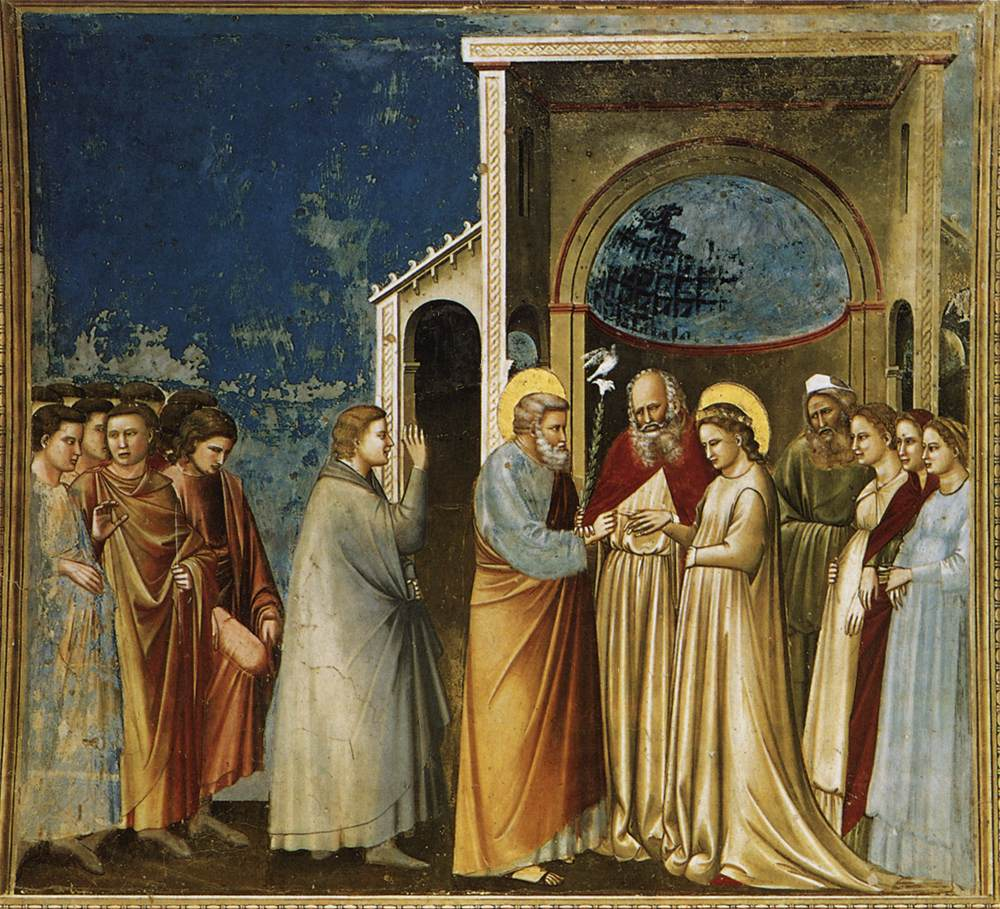
\includegraphics[width=7cm]{img/MariageGiotto.jpg}\end{center}
\subsection*{L'échange des consentements}

\emph{\rubrum Le prêtre s'adresse au fiancé :}
\textsc{Monsieur \textbf{Pierre-Henri Morille}, voulez-vous prendre pour légitime épouse Élisabeth Le Provost de Saint-Jean, ici présente, selon le rite de notre mère la Sainte Église?}
  
\emph{\rubrum Le fiancé répond : }\textsc{Oui, je le veux.}

\emph{\rubrum Puis, s'adressant à la fiancée :}
  \textsc{Mademoiselle \textbf{Élisabeth Le Provost de Saint-Jean}, voulez-vous prendre pour légitime époux Pierre-Henri Morille, ici présent, selon le rite de notre mère la Sainte Église?}
  
\emph{\rubrum La fiancée répond : }  \textsc{Oui, je le veux.}

\rubrica{Le prêtre invite alors les époux à se donner la main droite. Puis il confirme l'engagement dont il vient d'être témoin en disant :}

\versio{Ego conjungo vos in matrimonium, in nomine Patri, et Filii~\crux\ et Spiritui Sancti. Amen.}{Je vous déclare unis par le mariage au nom du Père et du Fils~\crux\ et du Saint Esprit. Ainsi soit-il.}
\newpage
\subsection*{La levée du voile}
\rubrica{Selon une tradition très ancienne, le nouvel époux lève le voile qui se trouve sur le visage de son épouse. Ce geste, très beau, signifie qu'un jour le Christ, qui est l'époux de l'Église, lèvera le voile qui pèse encore sur notre cœur et sur notre visage, et qu'alors nous le verrons face à face pour toujours. Ceci est un enseignement profond et grand sur le mystère du mariage parce que, précisément, l'amour humain est déjà le signe, la prophétie, qu'un jour Dieu nous épousera à l'intime de nous-même.}

\subsection*{Bénédiction des anneaux}
\rubrica{Le prêtre bénit les anneaux :}
\versio{%
\vb\ \crux Adiutórium nostrum in nómine Dómini.}{%
\vb\ \crux Notre secours est dans le nom du Seigneur.}
\reponsegras{%
\rb\ Qui fecit cælum et terram.}{%
\rb\ Qui a fait le ciel et la terre.}
\versio{%
\vb\ Dómine, exáudi oratiónem meam.}{%
\vb\ Seigneur, exaucez ma prière.}
\reponsegras{%
\rb\ Et clamor meus ad te véniat.}{%
\rb\ Et que mon cri s'élève jusqu'à vous.}
\versio{%
\vb\ Dóminus vobíscum.}{%
\vb\ Le Seigneur soit avec vous.}
\reponsegras{%
\rb\ Et cum spíritu tuo.}{%
\rb\ Et avec votre esprit.}
\versio{%
{\centering Orémus.\par}}{%
{\centering Prions.\par}}

\versio{Béne~\crux\ dic, Dómine, ánulos istos, quem nos in tuo nómine bene~\crux\ dícimus : ut,quæ eos gestáverint, fidelitátem íntegram ínvicem tenentes, in pace et voluntáte tua permáneant, atque in mútua caritáte semper vivant. Per Christum Dóminum nostrum.}
{Béni~\crux\ ssez, Seigneur, ces anneaux que nous béni~\crux\ ssons en votre nom, afin que ceux qui les porteront, les conservent dans une fidélité entière, demeurent dans la paix et dans votre volonté, et qu'ils vivent toujours dans une mutuelle affection. Par le Christ Notre-Seigneur.}
\reponsegras{\rb\ Amen.}{\rb\ Ainsi soit-il.}
\rubrica{Le prêtre asperge les anneaux d'eau bénite, puis l'époux passe au doigt de son épouse et à son doigt l'anneau qui ne les quittera plus.
Le prêtre bénit ce geste et appelle les grâces divines sur l'union irrévocable qui vient de se conclure.}

\subsection{Prière pour les époux}
\vspace*{0.5cm}
\versio{\vb\ Confírma hoc, Deus,quod operátus es in nobis.}{
\vb\ Confirmez, Seigneur, ce que vous avez accompli en nous.}

\reponsegras{\rb\ A templo sancto tuo, quod est in Jerúsalem.}{\rb\ De votre saint temple, en Jérusalem.}
\versio{Kýrie, éleison.}{Seigneur, ayez pitié de nous.}
\reponsegras{Christe, éleison. Kýrie, éleison.}{Christ, ayez pitié de nous. Seigneur, ayez pitié de nous.}

\versio{Pater noster}{Notre Père}
\rubrica{en silence jusqu'à :}
\versio{\vb\ Et ne nos indúcas in tentaiónem.}
{\vb\ Et ne nous laissez pas succomber à la tentation.}

\reponsegras{\rb\ Sed líbera nos a malo.}
{\rb\ Mais délivrez-nous du mal.}

\versio{\vb\ Salvos fac servos tuos.}{
\vb\ Seigneur, sauvez vos serviteurs.}

\reponsegras{\rb\ Deus meus, sperántes in te.}
{\rb\ Qui espèrent en vous, mon Dieu.}

\versio{\vb\ Mitte eis, Dómine, auxílium de sancto.}{\vb\ Envoyez-leur votre aide, Seigneur, de votre sanctuaire.}

\reponsegras{\rb\ Et de Sion tuére eos.}
{\rb\ Et de Sion, soutenez-les.}

\versio{\vb\ Esto eis, Dómine, turris fortitúdinis.}{\vb\ Soyez pour eux, Seigneur, comme une tour fortifiée.}

\reponsegras{\rb\ A fácie inimíci.}
{\rb\ Dressée contre l'ennemi.}

\versio{%
\vb\ Dómine, exáudi oratiónem meam.}{%
\vb\ Seigneur, exaucez ma prière.}
\reponsegras{%
\rb\ Et clamor meus ad te véniat.}{%
\rb\ Et que mon cri s'élève jusqu'à vous.}
\versio{%
\vb\ Dóminus vobíscum.}{%
\vb\ Le Seigneur soit avec vous.}
\reponsegras{%
\rb\ Et cum spíritu tuo.}{%
\rb\ Et avec votre esprit.}
\versio{\centering Orémus.\par}{\centering Prions.\par}
\versio{Réspice, qu\'æsumus, Dómine, super hos fámulos tuos: et institútis tuis, quibus propagatiónem humáni géneris ordinásti, benígnus assíste; ut qui te auctóre jungúntur, te auxiliánte servéntur. Per Christum Dóminum nostrum.}
{Jetez les yeux, Seigneur, sur ces époux vos serviteurs et protégez cette institution que vous avez établie pour la propagation du genre humain, afin qu'unis par vous ils soient également soutenus et gardés par votre secours. Par le Christ Notre-Seigneur.}
\reponsegras{%
\rb\ Amen.}{%
\rb\ Ainsi soit-il.}

\vspace*{\stretch{1}}
\begin{center}

\includegraphics[height=4cm]{img/SteFamille.pdf}
\end{center}
\vspace*{\stretch{1}}

%%%%%%%%%%%%%%%%%%%%%%%%%%%%%%%%%%%%%%%%%%%%%%%%%%%%%%%%%%%%%%%%%%%%%%%%%%%%%%%%%%%%%%%%%%%%
\chapter[]{\centering Messe de mariage}

\begin{center}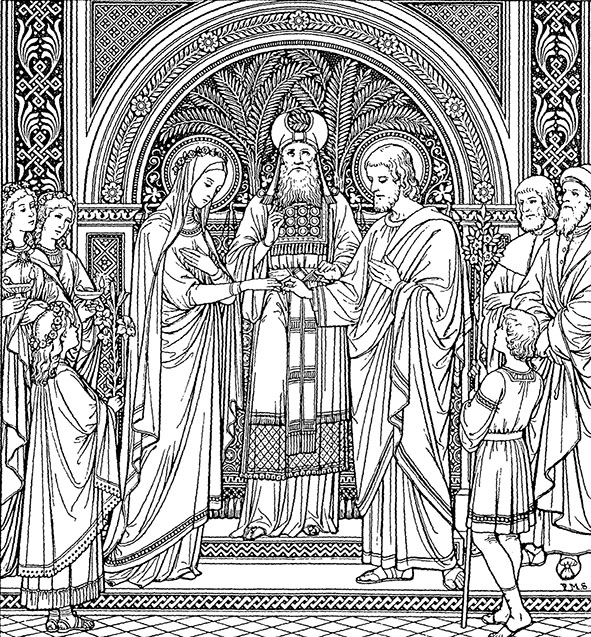
\includegraphics[width=7 cm]{img/MariageViergeLeger.jpg}\end{center}

\subsection*{Introït}
\rubrica{Pendant que le l'officiant se prépare à monter à l'autel avec les \emph{prières au bas de l'autel}, nous chantons l'Introït}
\versio{Deus Israël coniungat vos : et ipse sit vobiscum, qui misertus est duobus unicis : et nunc, Domine, fac eos plenius benedicere te.}
{Que le Dieu d'Israël vous unisse et qu'il reste avec vous, lui qui a eu pitié de deux enfants uniques ! Et maintenant, Seigneur, faites qu'ils reconnaissent de plus en plus vos bontés.}
\versio{\vb\ Beati omnes qui timent Dominum : qui ambulant in viis eius. \vb\ Glória Patri.}{Heureux tous ceux qui craignent le Seigneur, et qui marchent dans ses voies \vb\ Gloire au Père.}
\rubrica{On chante ensuite le \emph{Kyrie} et le \emph{Gloria} en alternance avec la chorale.}
\subsection*{Kyrie}
\cantus{Kyriale}{Kyrie-VIII}{}{5.}

\subsection*{Gloria}
\cantus{Kyriale}{Gloria-VIII-fideles}{}{5.}

%\includely{ly/MesseBleue/Abb-Jean-Robin-1920-2002-Kyrie}
%Kyrie eléison
%\cantus{Kyriale}{Christe-VIII1}{}{}
%Christe eléison
%\cantus{Kyriale}{Christe-VIII1}{}{}
%Kyrie eléison
%\cantus{Kyriale}{KYRIE-VIII2}{}{}
\subsection*{Collecte}
\versio{%
\vb\ Dóminus vobíscum.}{%
\vb\ Le Seigneur soit avec vous.}

\reponsegras{%
\rb\ Et cum spíritu tuo.}{%
\rb\ Et avec votre esprit.}

\versio{{\centering Orémus.\par}}
{{\centering Prions.\par}}
Écoutez-nous, Dieu tout-puissant et miséricordieux~: que votre bénédiction donne son plein achèvement à ce que nous venons d'accomplir en vertu de notre charge. Par Notre Seigneur.
\reponsegras{\rb\ Amen.}{\rb\ Ainsi soit-il.}

\rubrica{Mémoire de N.D. du Rosaire}
\versio{{\centering Orémus.\par}}
{{\centering Prions.\par}}
O Dieu, dont le Fils unique nous a obtenu le prix du salut éternel par sa vie, sa mort et sa résurrection ; faites, nous vous en prions, qu’honorant ces mystères au moyen du très saint Rosaire de la bienheureuse Vierge Marie, nous imitions ce qu’ils contiennent, et obtenions ce qu’ils promettent. Par le même Notre Seigneur.
\reponsegras{\rb\ Amen.}{\rb\ Ainsi soit-il.}
\newpage
\subsection*{Lecture de l'Épître de Saint Paul aux Éphésiens.}
\rubrica{Eph. 5, 22-33.}
Frères, que les femmes soient soumises à leur mari comme au Seigneur~; car le mari est le chef de la femme comme le Christ est le Chef de l'Église, qui est son Corps et dont il est le Sauveur. De même donc que l'Église est soumise au Christ, que les femmes le soient aussi à leur mari en toutes choses.
Vous, maris, aimez vos femmes tout comme le Christ a aimé l'Église et s'est livré pour elle, afin de la sanctifier en la purifiant par le baptême et la parole de vie~; il s'est ainsi préparé une Église resplendissante, sans tache, ni ride, ni rien de tel, mais sainte et irréprochable. Ainsi, les maris doivent aimer leur femme comme leur propre corps. Qui aime sa femme s'aime lui-même. Personne n'a jamais haï sa propre chair, mais il la nourrit et la soigne tout comme le Christ fait pour l'Église, puisque nous sommes les membres de son corps, formés de sa chair et de ses os.
C'est pourquoi l'homme quittera son père et sa mère pour s'attacher à sa femme, et les deux ne feront qu'une seule chair. Quel grand mystère~! Je veux dire par rapport au Christ et à l'Église. Ainsi donc, que chacun de vous aime sa femme comme soi-même, et que la femme ait pour son mari un affectueux respect.
\textbf{\rb\ Deo grátias.}
\subsection*{Graduel — Alleluia}
\rubrica{La Chorale chante ensuite le graduel et l'alleluia tiré des psaumes. 
%\emph{Le répons-graduel est emprunté au psaume 127, qui dépeint comme en une suave idylle les joies du sacrement de mariage.}(Bx Card. Schuster)
}
Votre femme sera comme une vigne féconde dans l’intérieur de votre maison. ℣. Vos enfants seront comme de jeunes plants d’olivier à l’entour de votre table.

Alléluia, alléluia. ℣. Que le seigneur vous envoie son secours de son sanctuaire : et que de Sion il vous protège. Alléluia.

\subsection*{Suite du saint Évangile selon Saint Matthieu.}
\rubrica{Matt. 19, 3-6.}
En ce temps-là, des pharisiens s'approchèrent de Jésus, et pour l'embarrasser lui dirent~: « Est-il permis à un homme de répudier sa femme pour n'importe quel motif~? » « N'avez-vous donc pas lu, répondit Jésus, que le Créateur, à l'origine, fit l'homme et la femme~? et qu'il a dit~: \emph{C'est pourquoi l'homme quittera son père et sa mère pour s'attacher à sa femme, et les deux ne seront qu'une seule chair}. Désormais, ils ne seront plus deux, mais ils seront un seul corps. Et par suite, ce que Dieu a uni, l'homme ne peut le séparer.»
\reponsegras{%
\rb\ Laus tibi Christe.}{%
\rb\ Christ, louange à vous.}
%%%%%%%%%%%%%%%%%%%%%%%%%%%%%%%%%
\newpage
\subsection*{\centering Offertoire}
\imagecentre{5cm}{consecration20.pdf}

\rubrica{À l'Offertoire l'Église offre le Corps et le Sang du Christ, représentés par le pain et le vin. Notre Seigneur a communiqué à son Église le pouvoir d'offrir le même sacrifice qu'il offrit sur la Croix. L'Église s'y unit comme victime. Nous sommes donc une seule victime avec le Christ, unissant nos propres offrandes et nos sacrifices à celui du Christ et de l'Église. Notre participation à cette offrande est exprimée par le chant de l'offertoire.}

J’ai espéré en vous, seigneur~: je vous ai dit~: Vous êtes mon Dieu~: mon sort est entre vos mains.

Recevez, Père saint, Dieu éternel et tout-puissant, cette offrande sans tache, que moi, votre indigne serviteur, je vous présente, à vous, mon Dieu vivant et vrai, pour mes péchés, offenses et négligences sans nombre, pour tous ceux qui m'entourent, ainsi que pour tous les fidèles vivants et morts~: qu'elle serve à mon salut et au leur pour la vie éternelle. Ainsi soit-il.

Dieu, ✠ qui, d'une manière admirable, avez créé la nature humaine dans sa noblesse, et l'avez restaurée d'une manière plus admirable encore, accordez-nous, selon le mystère de cette eau et de ce vin, de prendre part à la divinité de celui qui a daigné partager notre humanité, Jésus-Christ votre Fils, Notre Seigneur, qui, étant Dieu, vit et règne avec vous en l'unité du Saint-Esprit, dans tous les siècles des siècles. \mbox{Ainsi soit-il}.\looseness=1

\subsection*{Oraison}
Recevez nous, vous en prions, Seigneur, le don que nous vous offrons pour consacrer le lien du mariage~: et comme vous en êtes l’auteur, soyez-en aussi le gardien.
\newpage
\subsection*{%
Préface%
}


\rubrica{Par le chant de la Préface le prêtre rend grâces à Dieu au nom de l'Église pour l'œuvre du salut réalisée par Jésus-Christ.}

\versio{%
℣. Per ómnia sǽcula sæculórum.}{%
℣. Dans tous les siècles des siècles.}
\reponsegras{℟. Amen.}{℟. Ainsi soit-il.}
\versio{%
℣. Dóminus vobíscum.}{%
℣. Le Seigneur soit avec vous.}

\reponsegras{%
℟. Et cum spíritu tuo.}{%
℟. Et avec votre esprit.}

\versio{%
℣. Sursum corda.}{%
℣. Élevons nos cœurs.}

\reponsegras{%
℟. Habémus ad Dóminum.}{%
℟. Ils sont tournés vers le Seigneur.\looseness=-1}

\versio{%
℣. Grátias agámus Dómino Deo nostro.}{%
℣. Rendons grâces au Seigneur notre Dieu.}

\reponsegras{%
℟. Dignum et iustum est.}{%
℟. C'est juste et nécessaire.}
Il est vraiment juste et nécessaire, c’est notre devoir et c’est notre salut, de vous rendre grâces toujours et partout, Seigneur, Père saint, Dieu éternel et tout-puissant, par le Christ notre Seigneur.
Par lui les Anges louent votre majesté, les Dominations l’adorent, les Puissances la révèrent, les Cieux et les Forces des Cieux avec les bienheureux Séraphins la célèbrent, unis dans une même allégresse. A leurs chants nous vous prions de laisser se joindre aussi nos voix pour proclamer dans une humble louange :

\subsection*{Sanctus}
\rubrica{Alterné avec la chorale}
\cantus{Kyriale}{Sanctus-VIII-I}{5.}{}
Pleni sunt cæli et terra glória tua. Hosánna in excélsis !
\cantus{Kyriale}{Benedictus-VIII-I}{5.}{}
Hosánna in excélsis !
\newpage
\subsection*{\centering Consécration}
\imagecentre{5cm}{03preparatioAdMissam.jpg}

\rubrica{Le prêtre récite alors l'histoire de l'institution de l'Eucharistie en accomplissant les mêmes gestes que le Christ.}

\versio{%
Qui prídie quam paterétur, accépit panem in sanctas ac venerábiles manus suas, et elevátis óculis in cælum ad te Deum Patrem suum omnipoténtem, tibi grátias agens, bene ✠ díxit, fregit, dedítque discípulis suis, dicens~: Accípite, et manducáte ex hoc omnes.}{%
Celui-ci, la veille de sa Passion, prit du pain dans ses mains saintes et adorables, et, les yeux levés au ciel vers vous, Dieu, son Père tout-puissant, vous rendant grâces, il ✠ bénit ce pain, le rompit et le donna à ses disciples en disant~: Prenez et mangez-en tous.}


\rubrica{Le prêtre prononce alors les paroles mêmes de Notre-Seigneur. Par ces paroles il opère la conversion du pain au saint Corps du Christ.}

\versio{%
\scalebox{.91}[1]{\textsc{\addfontfeatures{Renderer=Basic}Hoc est enim Corpus meum.}}\par%
}{%
\textsc{\addfontfeatures{Renderer=Basic}Car ceci est mon Corps.}\par%
}

%\vspace{1\baselineskip plus 2\baselineskip}
\rubrica{Ces paroles étant prononcées, le prêtre fait la génuflexion pour adorer le saint Corps, l'élève pour le présenter à l'adoration des fidèles, puis reprend le récit de l'institution de l'eucharistie~:}

\versio{%
Símili modo postquam cenátum est, accípiens et hunc præclárum Cálicem in sanctas ac venerábiles manus suas~: item tibi grátias agens, bene ✠ díxit, dedítque discípulis suis, dicens~: Accípite, et bíbite ex eo omnes.}{%
De même, après le repas, il prit aussi ce précieux calice dans ses mains saintes et adorables, vous rendit grâces encore, le ✠ bénit et le donna à ses disciples en disant~: Prenez et buvez-en tous.}
\pagebreak
\rubrica{Prononçant alors les paroles mêmes de Notre-Seigneur, le prêtre opère la conversion du vin au précieux Sang du Christ.}
%
\nopagebreak\smallskip%
%
\versio{%
\textsc{\addfontfeatures{Renderer=Basic}Hic est enim Calix Sánguinis mei, novi et ætérni Testaménti~: mystérium fídei~: qui pro vobis et pro multis effundétur in remissiónem peccatórum.}%
}{%
\textsc{\addfontfeatures{Renderer=Basic}Car ceci est le Calice de mon Sang, le Sang de l'Alliance nouvelle et éternelle, le mystère de la foi, qui sera versé pour vous et pour un grand nombre en rémission des péchés.}%
}

\smallskip

\versio{%
Hæc quotiescúmque fecéritis, in mei memóriam faciétis.}{%
Toutes les fois que vous ferez cela, vous le ferez en mémoire de moi.}%

%\vspace{1\baselineskip plus 2\baselineskip}

\rubrica{Ces paroles étant prononcées, le prêtre fait la génuflexion pour adorer le précieux Sang. Il l'élève pour le présenter à l'adoration, et fait de nouveau la génuflexion.}

\subsection*{Communion}

\rubrica{%
  \emph{%
  Ô très grand amour de Dieu pour les hommes! À ceux qui l'avaient abandonné il a accordé un tel pardon, une telle part de grâces, qu'il se fait appeler Père.} (S. Cyrille de Jérusalem). Au nom de l'Église le Célébrant chante la prière que Jésus-Christ nous a apprise. Dans les rites latins, le Notre Père a toujours été chanté par le célébrant seul.}
\versio{%
  Orémus. Præcéptis salutáribus móniti, et divína institutióne formáti, audémus dícere :}{%
  Prions. Éclairés par le commandement du Sauveur et formés par l'enseignement d'un Dieu, nous osons dire~:}
\versio{%
  Pater noster, qui es in cælis : sanctificétur nomen tuum ; advéniat regnum tuum ; fiat volúntas tua sicut in cælo et in terra. Panem nostrum quotidiánum da nobis hódie ; et dimítte nobis débita nostra, sicut et nos dimíttimus debitóribus nostris. Et ne nos indúcas in tentatiónem.}{%
  Notre Père,qui êtes aux cieux, que votre nom soit sanctifié, que votre règne arrive, que votre volonté soit faite sur la terre comme au ciel. Donnez-nous aujourd'hui notre pain de chaque jour ; pardonnez-nous nos offenses comme nous pardonnons à ceux qui nous ont offensés ; et ne nous laissez pas succomber à la tentation.}
\rubrica{On répond :}  
%\reponsegras{%
%\rb\ Sed líbera nos a malo.}{%
%\rb\ Mais délivrez-nous du mal.}
\parbox{7cm}{
\cantus{Verset}{SedLiberaNos}{}{}
} Mais délivrez-nous du mal.
{\begin{center} \greseparator{1}{20}\end{center}}

\newpage
%%%%%%%%%%%%%%%%%%%%%%%%%%%%%%
\section*{\centering Bénédiction nuptiale}
\rubrica{Tout de suite après le \emph{Pater}, le prêtre se tourne vers les nouveaux époux (seuls agenouillés) et procède à la bénédiction nuptiale solennelle.}

\versio {%
{\centering Orémus.\par}
Propitiáre, Dómine, supplicatiónibus nostris, et institútis tuis, quibus propagatiónem humáni géneris ordinásti, benígnus assíste~: ut, quod te auctóre iúngitur, te auxiliánte servétur. Per Dóminum nostrum Iesum Christum Fílium tuum, qui tecum vivit et regnat in unitáte Spíritus Sancti Deus, per ómnia s\'æcula sæculórum.}{%
{\centering Prions.\par}
Seigneur, soyez favorable à nos supplications et accordez votre assistance bienveillante à cette institution du foyer, destinée à assurer la propagation du genre humain, afin que ceux qui s'unissent sous votre autorité soient gardés par votre secours. Par Notre Seigneur Jésus-Christ votre Fils, qui étant Dieu vit et règne avec vous en l'unité du Saint-Esprit, dans tous les siècles des siècles.}
\reponsegras{\rb\ Amen.}{\rb\ Ainsi soit-il.}

\versio{{\centering Orémus.\par}
Deus, qui potestáte virtútis tuæ de níhilo cuncta fecísti~: qui dispósitis universitátis exórdiis, hómini ad imáginem Dei facto, ídeo inseparábile mulíeris adiutórium condidísti, ut femíneo córpori de viríli dares carne princípium, docens quod ex uno placuísset instítui, nunquam licére disiúngi~: }{%
{\centering Prions.\par}
 Dieu, qui par votre toute-puissance avez fait de rien toutes choses~; qui avez disposé harmonieusement les commencements de l'univers~; qui, ayant créé l'homme à l'image de Dieu, avez fait de la femme son aide inséparable, et avez donné pour origine à son corps la chair de l'homme, enseignant par là qu'il n'est jamais permis de séparer ceux qu'il vous a plu de créer dans l'unité~; }
\versio{Deus, qui tam excellénti mystério coniugálem cópulam consecrásti, ut Christi et Ecclésiæ sacraméntum præsignáres in f\'\oe dere nuptiárum~:}
{Ô Dieu qui, donnant au lien conjugal une consécration mystérieuse et sublime, avez fait du contrat nuptial le symbole de l'union sainte du Christ et de l'Église~; }
\versio{Deus, per quem múlier iúngitur viro, et socíetas principáliter ordináta ea benedictióne donátur, quæ sola nec per originális peccáti p\oe nam, nec per dilúvii est abláta senténtiam~: }
{Ô Dieu, par qui la femme est unie à l'homme et de qui cette association, principe de l'ordre humain, reçoît la seule bénédiction que n'ont abolie ni le châtiment du péché originel, ni la condamnation du déluge~;}

\versio{Réspice propítius super hanc fámulam tuam, quæ maritáli iungénda consórtio, tua se éxpetit protectióne muníri~: }
{Regardez avec bienveillance votre servante ici présente~; avant de s'unir à son époux par le mariage, elle demande le soutien de votre protection.} 
\versio{Sit in ea iugum dilectiónis et pacis~: fidélis et casta nubat in Christo, imitatríxque sanctárum permáneat feminárum~: sit amábilis viro suo, ut Rachel~: sápiens, ut Rebécca~: long\'\ae va et fidélis, ut Sara~: }
{Que la loi de sa vie soit l'amour et la paix~; qu'elle se marie en Jésus-Christ, dans la fidélité et la chasteté, et qu'elle persévère dans l'imitation des saintes femmes d'autrefois~; qu'elle soit aimable à son époux comme Rachel, sage comme Rébecca, fidèle au cours d'une longue vie comme Sara.}
\versio{Nihil in ea ex áctibus suis ille auctor prævaricatiónis usúrpet~: nexa fídei, mandatísque permáneat~: uni thoro iuncta, contáctus illícitos fúgiat~: múniat infirmitátem suam róbore disciplínæ~: sit verecúndia gravis, pudóre venerábilis, doctrínis cæléstibus erudíta~: sit fecúnda in sóbole, sit probáta et ínnocens~:}
{Que le démon, auteur du péché, ne lui inspire aucune des actions mauvaises par lesquelles il usurpe les droits de Dieu. Qu'elle reste attachée à la foi et aux commandements~; qu'elle ne laisse rien d'illicite effleurer sa fidélité inviolée~; qu'elle appuie sa fragilité sur une forte discipline de vie~; que sa modestie commande l'estime, sa pudeur le respect, qu'elle soit instruite dans la science qui vient du Ciel. Qu'elle soit une mère féconde~; qu'elle soit vertueuse et pure~;} 
\versio{Et ad beatórum réquiem, atque ad cæléstia regna pervéniat~: et vídeant ambo fílios filiórum suórum, usque in tértiam et quartam generatiónem, et ad optátam pervéniant senectútem. Per eúndem Dóminum nostrum Iesum Christum Fílium tuum, qui tecum vivit et regnat in unitáte Spíritus Sancti Deus, per ómnia s\'æcula sæculórum.}
{Et qu'elle parvienne au repos des élus et au céleste Royaume. Que ces nouveaux époux voient les enfants de leurs enfants jusqu'à la troisième et à la quatrième génération, et arrivent à une heureuse vieillesse. Par Notre Seigneur Jésus-Christ votre Fils, qui étant Dieu vit et règne avec vous en l'unité du Saint-Esprit, dans tous les siècles des siècles. }
\reponsegras{\rb\ Amen.}{\rb\ Ainsi soit-il.}
{\begin{center} \greseparator{1}{20}\end{center}}
%\begin{center}
\includegraphics[height=3cm]{img/AMDG.png}\end{center}
%%%%%%%%%%%%%%%%%%%%%%%%
\newpage
\rubrica{Le prêtre continue alors la messe, avec la fraction de l'hostie}
\versio{%
℣. Per ómnia sǽcula sæculórum.}{%
℣. Dans tous les siècles des siècles.}

\versio{%
℟. Amen.}{%
℟. Ainsi soit-il.}
%
\versio{%
℣. Pax ✠ Dómini sit ✠ semper vobís ✠ cum.}{%
℣. La paix ✠ du Seigneur soit ✠ toujours avec ✠ vous.}
%
\versio{%
℟. Et cum spíritu tuo.}{%
℟. Et avec votre esprit.}

\rubrica{Le mélange d'une parcelle de l'hostie dans le précieux Sang signifie l'unité de tous dans le même sacrifice.}

\subsection*{Agnus Dei}
\rubrica{Alterné avec la chorale.}
\versio{%
Agnus Dei, qui tollis peccáta mundi, miserére nobis.%
}{%
Agneau de Dieu, qui ôtez les péchés du monde, ayez pitié de nous.%
}%
\cantus{Kyriale}{Agnus-VIII-2}{6.}{}
\versio{%
Agnus Dei, qui tollis peccáta mundi, dona nobis pacem.%
}{%
Agneau de Dieu, qui ôtez les péchés du monde, donez-nous la paix.%
}%


\rubrica{Aux messes solennelles, l'oraison suivante pour la paix est suivie du baiser de paix.}
Seigneur Jésus-Christ, qui avez dit à vos Apôtres : C'est la paix que je vous laisse en héritage, c'est ma paix je vous donne, ne regardez pas mes péchés, mais la foi de votre Église~; daignez, selon votre volonté, lui donner la paix et la rassembler dans l'unité, vous qui, étant Dieu, vivez et régnez dans tous les siècles des siècles. Ainsi soit-il.

\rubrica{Le baiser de paix, manifestant l'union dans la paix du Christ, est hiérarchiquement transmis de l'autel jusqu'au dernier degré du clergé. \emph{Ne pense pas que ce baiser soit comme ceux qui se donnent sur la place entre amis ordinaires. Il unit les âmes entre elles~; il est réconciliation, et pour cette raison il est saint.} (S.~Cyrille de Jérusalem)}

\subsection*{Communion}
Seigneur Jésus-Christ, Fils du Dieu vivant, qui, accomplissant la volonté du Père dans une œuvre commune avec le Saint-Esprit, avez par votre mort donné la vie au monde, délivrez-moi par votre Corps et votre Sang infiniment saints de tous mes péchés et de tout mal. Faites que je reste toujours attaché à vos commandements, et ne permettez pas que je sois jamais séparé de vous, qui, étant Dieu, vivez et régnez avec Dieu le Père et le Saint-Esprit dans les siècles des siècles. Ainsi soit-il.

Seigneur Jésus-Christ, si j'ose recevoir votre Corps malgré mon indignité, que cela n'entraîne pour moi ni jugement ni condamnation, mais, par votre miséricorde, me serve de sauvegarde et de remède pour l'âme et pour le corps, vous qui, étant Dieu, vivez et régnez avec Dieu le Père en l'unité du Saint-Esprit, dans tous les siècles des siècles. Ainsi soit-il.

\rubrica{Après avoir communié, le prêtre se retourne vers les fidèles en leur présentant le saint Corps du Christ.}

\versio{%
Ecce Agnus Dei, ecce qui tollis peccáta mundi.}{%
Voici l'Agneau de Dieu, voici celui qui enlève les péchés du monde.}

\rubrica{Nous répondons par les paroles du bienheureux centurion. Cette fois ce n'est plus la guérison d'un serviteur que nous demandons, mais celle de notre âme.}
%
\reponsegras{%
Dómine, non sum dignus, ut intres sub tectum meum~: sed tantum dic verbo, et sanábitur ánima mea. \emph{ter}}{%
Seigneur, je ne suis pas digne que vous entriez sous mon toit~; mais dites seulement une parole, et mon âme sera guérie. \emph{ter}}

\begin{framed}
\rubrica{Aux premiers siècles le diacre invitait ceux qui ne pouvaient pas communier à se retirer. Aujourd'hui l'Église est plus indulgente mais les conditions pour communier sont les mêmes~:}
\begin{itemize}

\item être baptisé et catholique~; 
\item ne pas avoir de péché mortel sur la conscience, ce qui suppose notamment l'observation des lois de l'Église au sujet du mariage~; 
\item avoir observé le jeûne eucharistique. La discipline actuelle est d'une heure de jeûne avant la communion (nous conseillons cependant de s'en tenir à la discipline d'avant le Concile Vatican II~: trois heures pour la nourriture solide, une heure pour le liquide non alcoolisé).
\end{itemize}

La sainte communion est reçue à genoux et directement dans la bouche.
\end{framed}

\needspace{3\baselineskip}
\rubrica{En donnant la sainte Eucharistie, le prêtre dit~:}

\versio{%
Corpus Dómini nostri Iesu Christi custódiat ánimam tuam in vitam ætérnam. Amen.}{%
Que le Corps de Notre Seigneur Jésus-Christ garde votre âme pour la vie éternelle. Ainsi soit-il.}

\rubrica{%
On ne répond rien.}

\rubrica{%
Jésus-Christ est le Bon Pasteur qui donne sa vie pour ses brebis. \emph{Je suis venu pour qu'ils aient la vie et qu'ils l'aient en abondance}. Il nous communique cette vie dans la sainte Eucharistie.%
}

\subsection*{Chant de communion}
\rubrica{Ps. 127, 4 et 6.}
Voilà comment sera béni tout homme qui craint le Seigneur. Puisses-tu voir les enfants de tes enfants ! Que la paix soit sur Israël !

\subsection*{Postcommunion}
\versio{%
\vb\ Dóminus vobíscum.}{%
\vb\ Le Seigneur soit avec vous.}

\reponsegras{\rb\ Et cum spíritu tuo.}{\rb\ Et avec votre esprit.}
\versio{Qu\'æsumus, omnípotens Deus~: institúta providéntiæ tuæ pio favóre comitáre~: ut, quos legítima societáte connéctis, longæva pace custódias. Per Dóminum nostrum Iesum Christum Fílium tuum, qui tecum vivit et regnat in unitáte Spíritus Sancti Deus, per ómnia s\'æcula sæculórum.}
{Nous vous en prions, Dieu tout-puissant, accompagnez de votre paternelle bienveillance ce qu'a établi votre providence~: gardez dans la paix, jusqu'à un grand âge, ceux dont vous nouez l'union sacrée. Par Notre Seigneur Jésus-Christ votre Fils, qui étant Dieu vit et règne avec vous en l'unité du Saint-Esprit, dans tous les siècles des siècles.}

\subsection*{Bénédiction de la nouvelle épouse}
\rubrica{Avant de bénir les fidèles, le prêtre donne une bénédiction spéciale à la nouvelle épouse}
\versio{Deus Abraham, Deus Isaac, et Deus Iacob sit vobíscum~: et ipse adímpleat benedictiónem suam in vobis~: ut videátis fílios filiórum vestrórum usque ad tértiam et quartam generatiónem, et póstea vitam ætérnam habeátis sine fine~: adiuvánte Dómino nostro Iesu Christo, qui cum Patre et Spíritu Sancto vivit et regnat Deus, per ómnia s\'æcula sæculórum.}{%
Que le Dieu d'Abraham, le Dieu d'Isaac, le Dieu de Jacob soit avec vous et que lui-même vous comble de sa bénédiction, afin que vous puissiez voir les enfants de vos enfants jusqu'à la troisième et la quatrième génération, et qu'ensuite vous possédiez sans fin la vie éternelle, avec l'aide de Notre Seigneur Jésus-Christ, qui, étant Dieu, vit et règne avec le Père et le Saint-Esprit dans tous les siècles des siècles.}

\reponsegras{%
\rb\ Amen.}{%
\rb\ Ainsi soit-il.}

\rubrica{%
Le prêtre asperge d'eau bénite les nouveaux époux, puis il donne la bénédiction finale à tous~:}

\versio{%
Benedícat vos omnípotens Deus, Pater, et ✠ Fílius, et Spíritus Sanctus.}{%
Que Dieu tout-puissant vous bénisse, le Père, ✠ le Fils et le Saint-Esprit.}
\reponsegras{%
\rb\ Amen.}{%
\rb\ Ainsi soit-il.}

{\begin{center} \greseparator{1}{20}\end{center}}
\newpage
\section[]{Consécration à la Vierge}
\rubrica{Les époux vont consacrer leur nouveau foyer à la Vierge, et signer les registres avec le célébrant et les témoins, pendant ce temps, on chante l'hymne suivant en alternance avec la chorale :}
%\titre{Ave Maris stella}
\cantus{Hymne}{AveMarisStella}{1.}{Hymn.}
\noindent
\vulgo{1. Salut, étoile de la mer, Mère de Dieu féconde, Salut, ô toujours Vierge, Porte heureuse du ciel !}

\versio{2. Sumens illud Ave~\newline
Gabriélis ore,~\newline
Funda nos in pace,~\newline
Mutans Hevæ nomen.}
{2. Vous qui de Gabriel~\newline
Avez reçu l'Ave,~\newline
Fondez-nous dans la paix,~\newline
Changeant le nom d'Ève~}

\versio{3. Solve vincla reis,~\newline
Profer lumen cæcis,~\newline
Mala nostra pelle,~\newline
Bona cuncta posce.}
{3. Délivrez les captifs,~\newline
Éclairez les aveugles,~\newline
Chassez loin tous nos maux,~\newline
Demandez tous les biens.}

\versio{4. Monstra te esse matrem,~\newline
Sumat per te preces,~\newline
Qui pro nobis natus~\newline
Tulit esse tuus.}
{4. Montrez en vous la Mère,~\newline
Vous-même offrez nos v{\oe}ux~\newline
Au Dieu qui, né pour nous,~\newline
Voulut naître de vous.}

\versio{5. Virgo singuláris,~\newline
Inter omnes mitis,~\newline
Nos, culpis solútos,~\newline
Mites fac et castos.}
{5. O Vierge incomparable,~\newline
Vierge douce entre toutes,~\newline
Affranchis du péché,~\newline
Rendez-nous doux et chastes.}

\versio{6. Vitam præsta puram,~\newline
Iter para tutum,~\newline
Ut, vidéntes Iesum,~\newline
Semper collætémur.}
{6. Donnez une vie pure,~\newline
Préparez un chemin sûr,~\newline
Pour que voyant Jésus~\newline
Notre liesse soit éternelle.}

\versio{7. Sit laus Deo Patri,~\newline
Summo Christo decus,~\newline
Spirítui Sancto,~\newline
Tribus honor unus.~ Amen.}
{7. Louange à Dieu le Père,~\newline
Gloire au Christ souverain,~\newline
Louange au Saint-Esprit,~\newline
Aux trois un seul hommage. Amen.}

\subsubsection*{\centering \Large{Consécration du foyer à la Très sainte Vierge Marie}}
\newfontfamily\malettrine[Scale=0.8]{l800}
\renewcommand{\LettrineFontHook}{\malettrine\color{black}}
\vspace*{\stretch{1}}
\large{
\lettrine{E}{n ce jour solennel, nous vous saluons,} Ô Reine du ciel et de la terre, et devant
toute la cour céleste, en présence de Dieu Tout Puissant, Père, Fils et Saint-Esprit,
nous vous consacrons, aujourd'hui, nos deux corps et nos deux âmes.

Ô Marie Immaculée, Vierge de lumière, Étoile du matin, daignez s'il vous plaît,
nous bénir et nous couvrir de votre maternelle protection.

Ô Mère du bon conseil, renforcez sans cesse notre union et faites de notre maison,
Mère de la divine grâce, une demeure de paix, de bonheur simple et de pureté.

Ô Mère Admirable, apprenez-nous à nous donner l'un à l'autre chaque jour, et à
pratiquer la volonté de Dieu dans une foi profonde, une espérance ferme et une
charité sans borne, dans un total abandon à la divine Providence.

Ô Refuge assuré des pécheurs, exaucez les désirs de vos humbles serviteurs,
prosternés en ce jour devant vous.

Dans l'épreuve, rappelez-nous, Ô Notre-Dame
des Sept-Douleurs, que le chemin ici-bas, passe par Jésus crucifié. Aidez-nous,
Mère du Christ, à être fidèles à notre engagement jusqu'à la mort.


Soyez la Reine de nos enfants, Mère Admirable, soyez notre soutien, Mère sans
tâche, pour les élever dans l'amour et la crainte de Dieu.
Ô Reine du Très Saint Rosaire, Rose mystique, Tour de David, Maison d'or,
Arche d'alliance, restez à nos côtés, et soyez notre refuge maternel jusqu'à notre
dernier soupir.

Et, dans votre suprême bonté, Vase Spirituel, Porte du Ciel,
reformez au Paradis notre foyer d'ici-bas, consacré à jamais à votre Coeur
immaculé. Ainsi soit-il.}
\imagecentre{3cm}{Frise.pdf}
\vspace*{\stretch{1}}
\newpage
\subsection*{Action de grâces — Magnificat}
\rubrica{Le Magnificat est alterné avec la chorale}
\cantus{Psaume}{Intonation-Magnificat-6-royal}{5.}{}
{1. Mon âme Exalte le Seigneur}
\psalmusversio[tonus=6F-alt,monprimus=2]{Magnificat-bilingue}
\mongloria[tonus=6F-alt]{}
\newpage
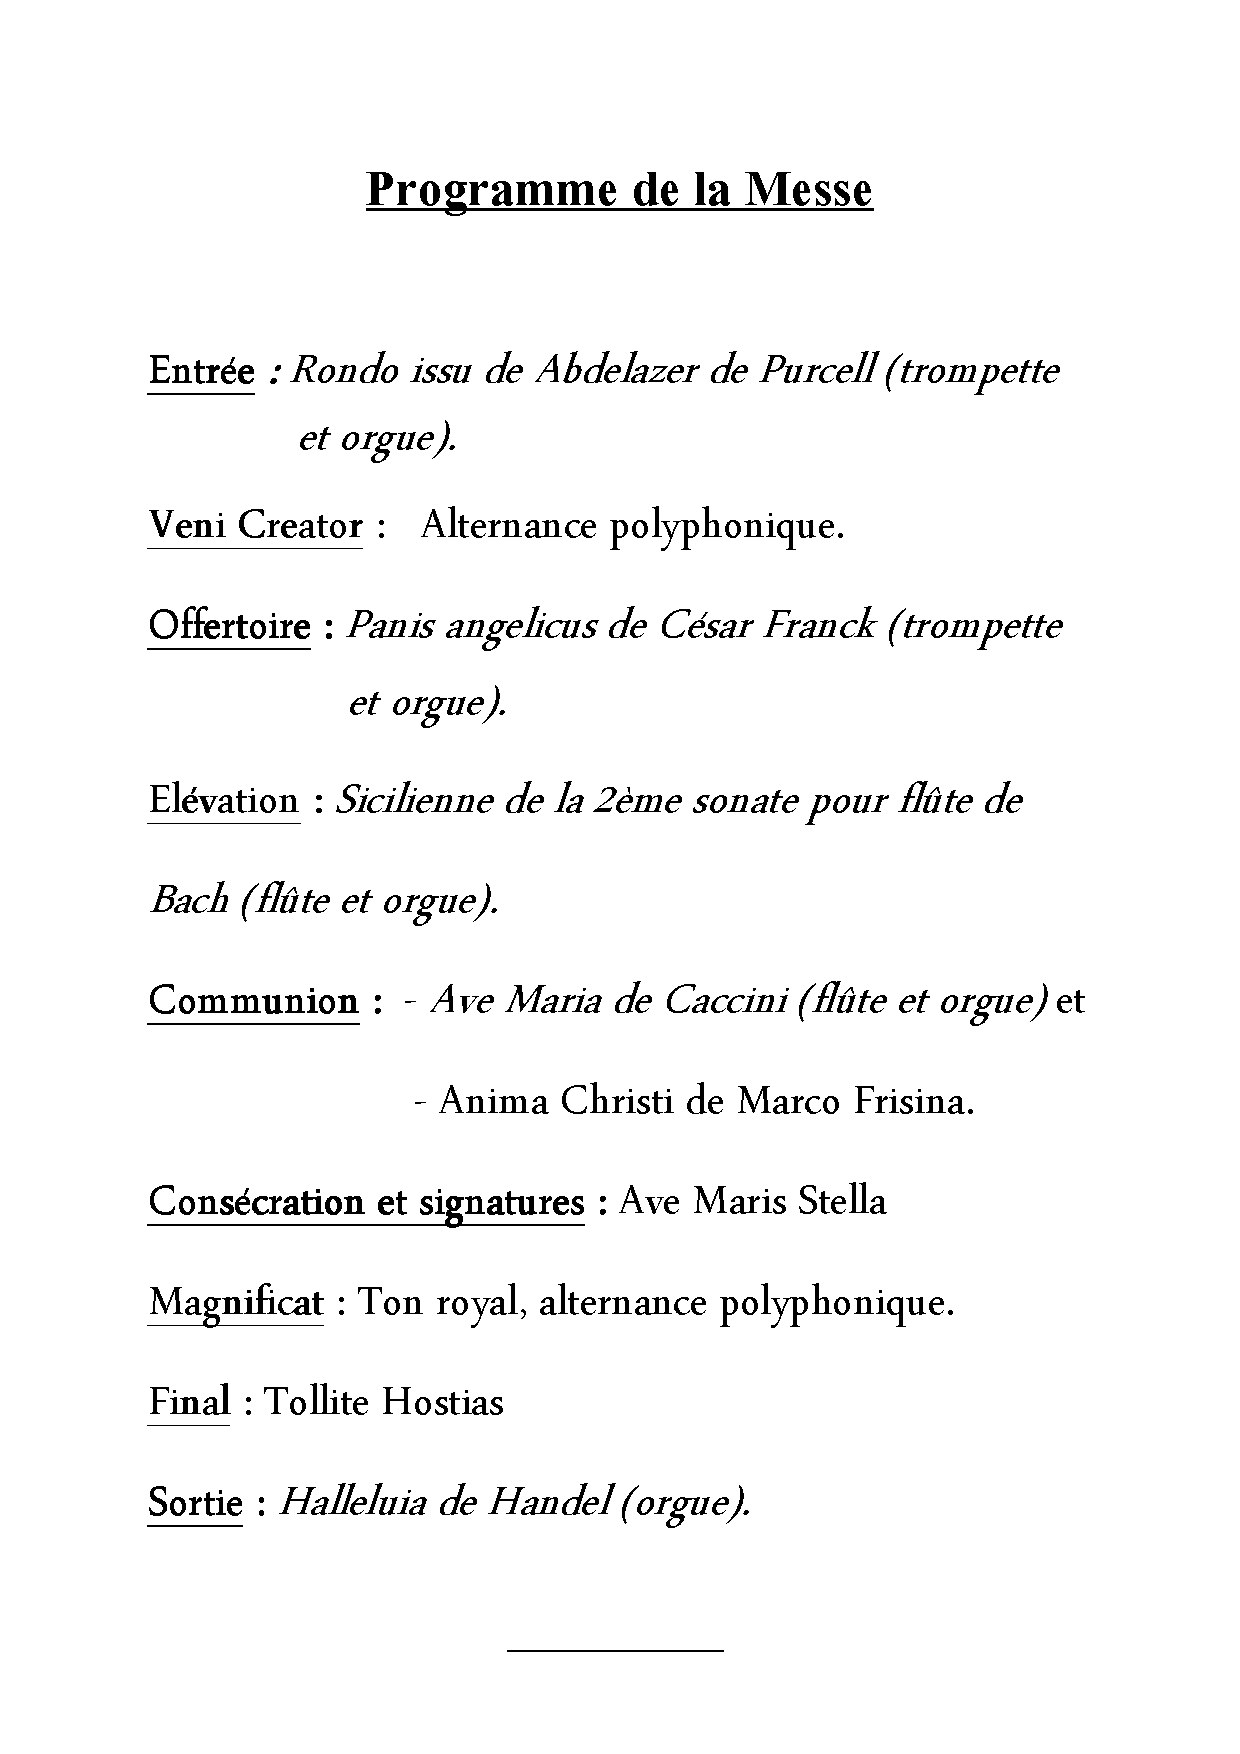
\includepdf{pdf/Programme.pdf}
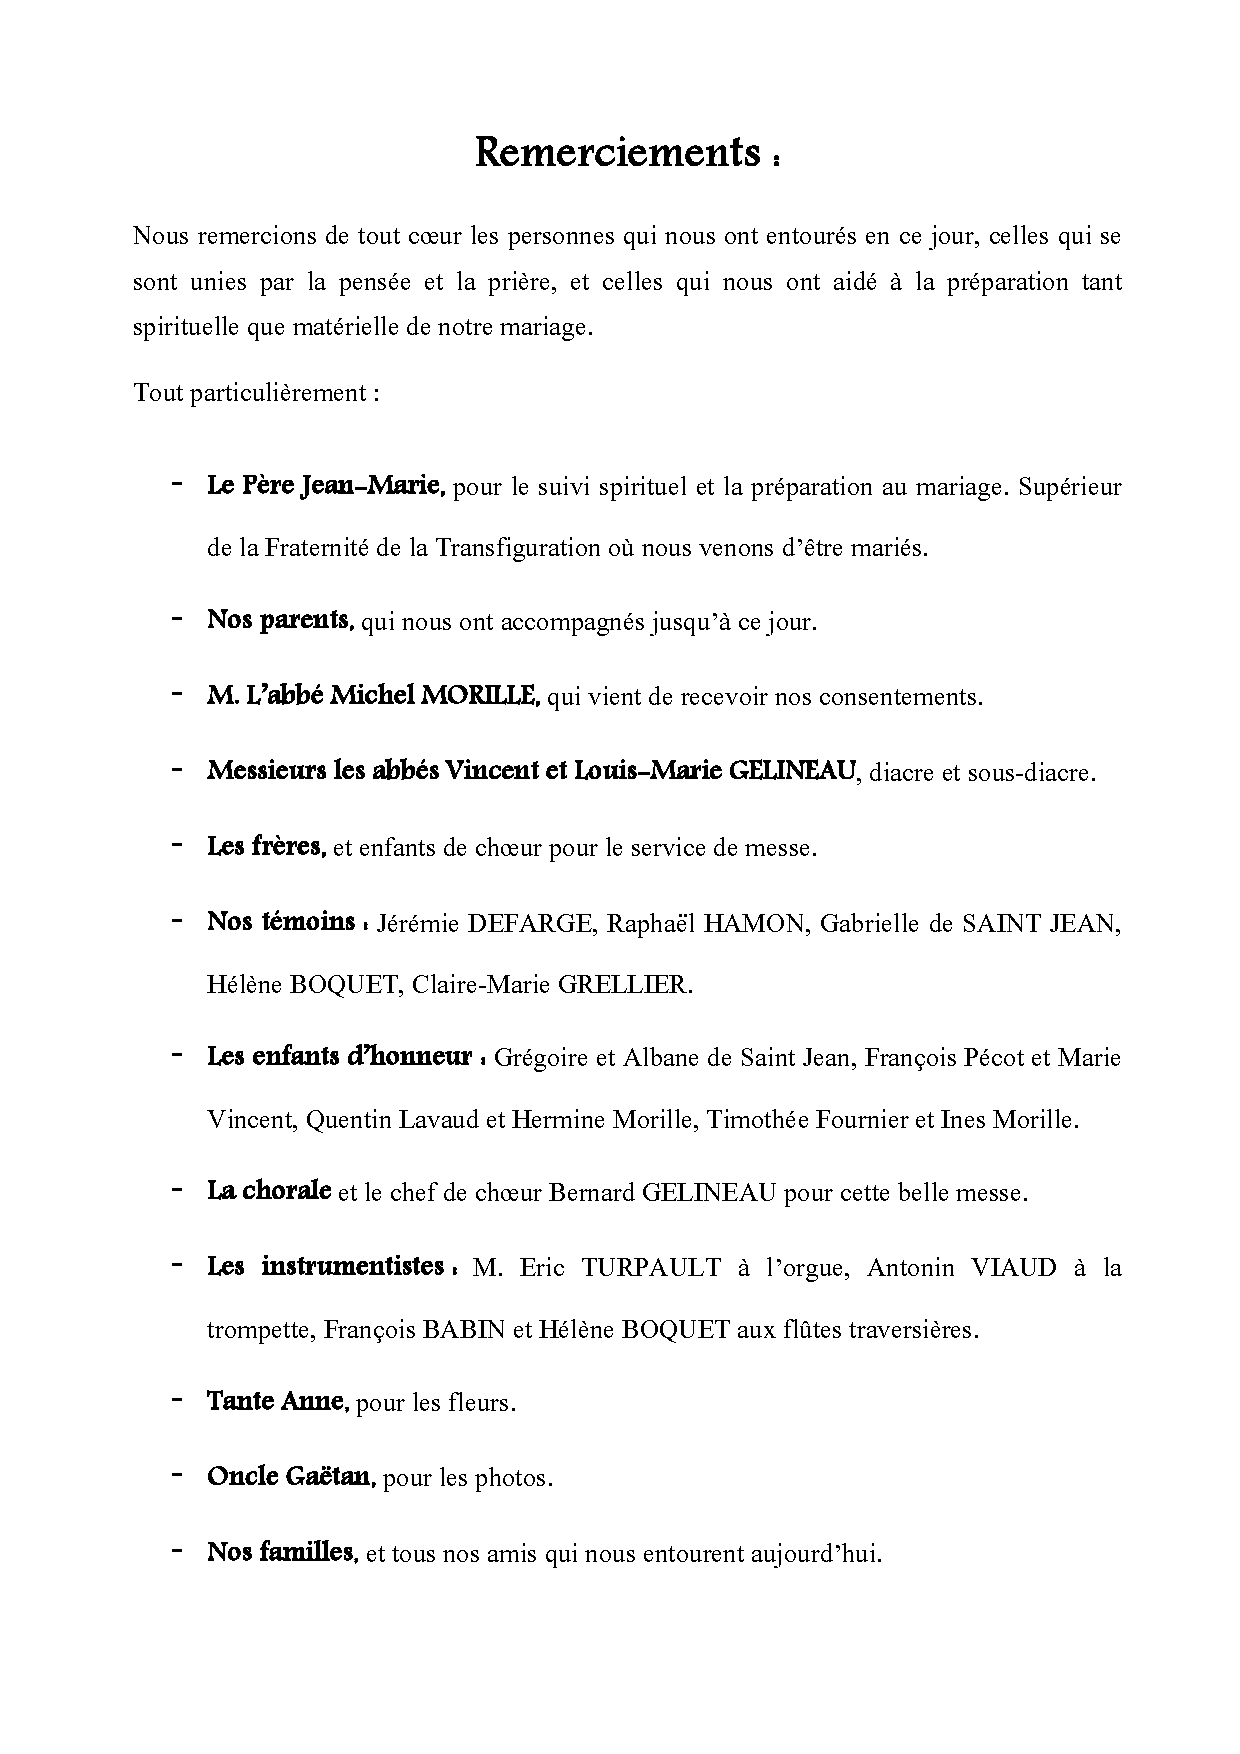
\includepdf{pdf/Remerciements.pdf}
\end{document}